\chapter{Implementation Keypoints }
\label{sec:implementation_keypoints}

This chapter gives an overview of the keypoints regarding the implementation of the methods illustrated in Chapter \ref{sec:algorithm_concepts}.

\section{2D-RRT*}

The RRT* path planner was firstly implemented on a 2D plane. 

\subsection{Runtime Improvement}

The main challenge here was the runtime, which increases exponentially with the number of iterations. As a reference, one of the first implemented versions took approximately 30 minutes to compute 10'000 iterations. This is due to the following reasons:

\begin{itemize}
	\item
	The collision-check function takes two states as an input and scans single points along the connection on collision with a specific check resolution. As one can see in Figure \ref{pics:obstacle_detection}, the smaller the resolution gets, the higher the probability of detecting a potential threat is. However, a small resolution results in long runtime for the collision-check function. Since this function gets called at least once per iteration, it has strong influence on the overall calculation time of the path planner. 
	\item
	At high amount of configurations in the workspace, the search of the nearest neighbour as well as the search of potential neighbours for the rewiring step becomes time-consuming, since the algorithm has to check the distance to each available state one by one.  	
\end{itemize} 

\begin{figure} [h]
	\centering
	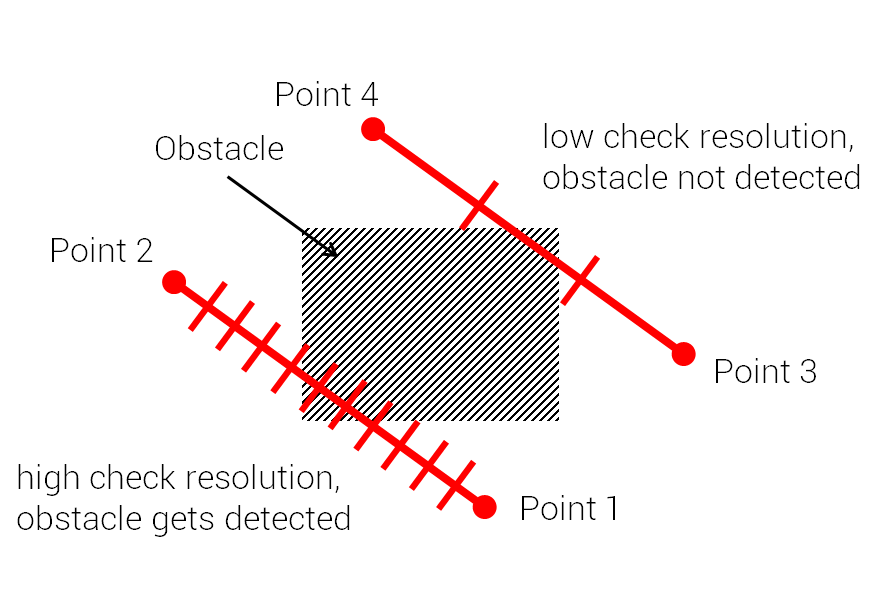
\includegraphics[width=0.75\textwidth]{images/obstacle_detection.png}
	\caption{Influence of the check resolution on obstacle detection.}
	\label{pics:obstacle_detection}
\end{figure}

Both problems can be kept within a limit by the implementation of the variable search radius described in Chapter \ref{(sec: rrt*)}. Regarding the collision-check function, the runtime could be improved by increasing the check resolution. However, this would take place at the expense of safety and is thus not recommendable.\\  

\subsubsection{k-d-tree}

A method called k-dimensional-tree (k-d-tree) can be used to reduce the searching work. It is a data-structure for organizing k-dimensional points by their attributes. As in the example of Figure \ref{pics:kd_tree}, the idea is to divide the configuration space into smaller subgroups. This is done by repeatedly splitting the space at the median of different attributes, which can be represented by a tree. By arrival of a new point, it only needs to be sorted based on its attributes into the corresponding subgroup. This way, the search can be restricted and the runtime improved. This method is an approximating technique and in some cases, errors in the search of the nearest neighbour can occur. In \textit{MATLAB}, k-d-tree is already implemented in the Statistics and Machine Learning Toolbox\footnote{http://ch.mathworks.com/help/stats/index.html}.

 
\begin{figure} [h]
	\centering
	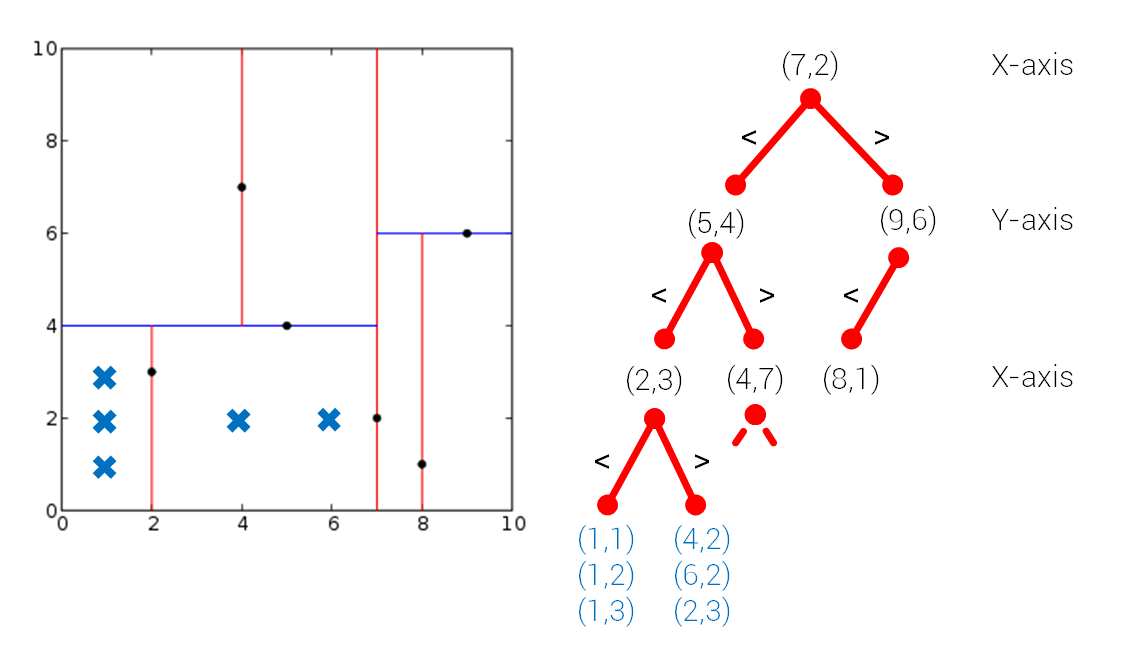
\includegraphics[width=1\textwidth]{images/kd-tree.png}
	\caption{Example of a 2-d-tree.}
	\label{pics:kd_tree}
\end{figure}

\subsubsection{Matrix Operation}

Since \textit{MATLAB} is designed for numerical calculation using matrices, the run time can be minimized by using matrix operations instead of for-loops. In the following, two code parts are shown which shows the search for the nearest state (see Code \ref{matrix_op1}) and the neighbours (see Code \ref{matrix_op2}). Furthermore, a runtime test showed that matrix operations is slightly more time-efficient at high iteration number than k-d-tree (see figure \ref{pics:runtime}).

\begin{figure} [h]
	\centering
	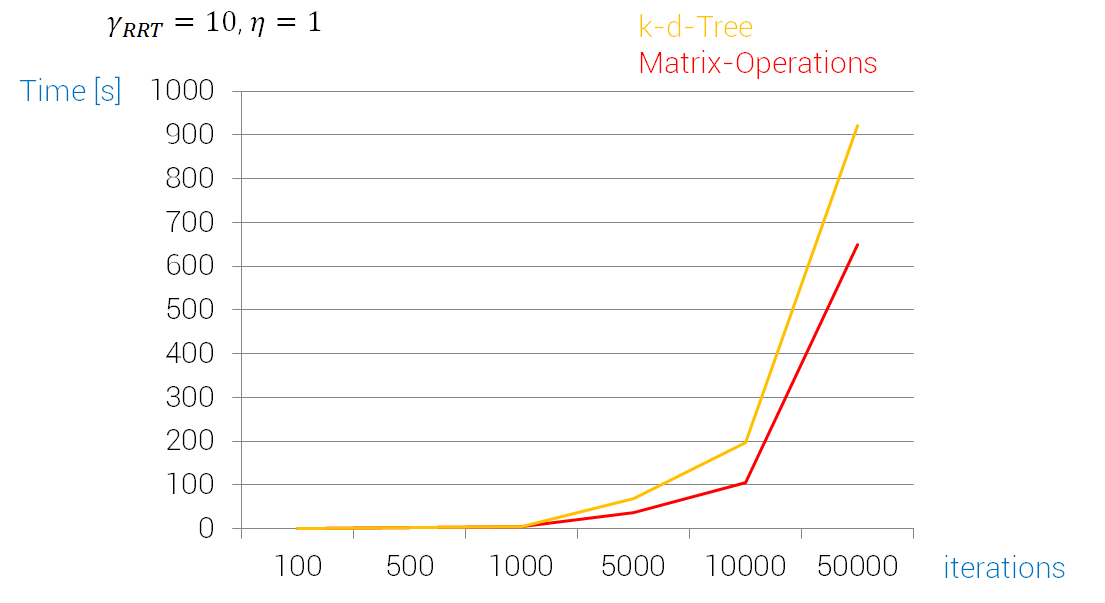
\includegraphics[width=1\textwidth]{images/runtime.png}
	\caption{Calculation time: k-d-tree and Matrix Operations in comparison}
	\label{pics:runtime}
\end{figure}

\begin{lstlisting}[caption={Nearest State Search},label=matrix_op1]
difference_array=states_array(:,1:2)-repmat([x_sample,y_sample],size(states_array,1),1);

distance_array=sqrt(sum(difference_array.^2,2));

[~,idx]=ismember(min(distance_array),distance_array);
\end{lstlisting}

\begin{lstlisting}[caption={Neighbours Search},label=matrix_op2]
distance_array=states_array(:,1:2)-repmat([states_array(i,1),states_array(i,2)],size(states_array,1),1);
        
distance_from_neighbor=sqrt(sum(distance_array.^2,2));
        
neighbors=find(distance_from_neighbor<=search_radius);
\end{lstlisting}

\subsection{Path Curvature}

In a further step, the influence of the cost function on the curvature of the path was evaluated. Both, the euclidean distance as well as the angular change between line segments were considered with corresponding weight-factors in the step cost function (see formula \ref{eq:cost_function}). The angle between two connections were considered in square in order to penalize large angular changes.

\begin{figure} [h]
	\centering
	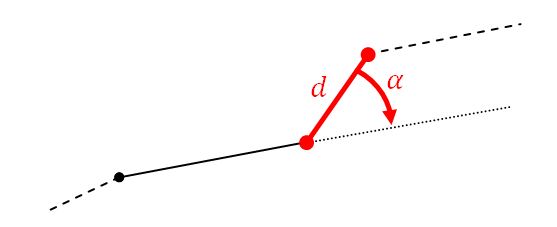
\includegraphics[width=0.6\textwidth]{images/angle.png}
	\caption{Angle $\alpha$ between two connections and distance d.}
	\label{pics:angle}
\end{figure}

\begin{equation}
cost_{step} = w_{1}\,d+w_{2} \,\alpha^{2}
\label{eq:cost_function}
\end{equation} 

\section{3D-RRT*}

The implemented algorithms and functions for the 2D plane was adapted for the 3D configuration space. The main problem was the implementation of a 3D occupancy grid, which will be illustrated in the following section.    

\subsection{3D Occupancy Grid}
Since \textit{Octomap}\footnote{3D mapping framework based on octrees.} does not exist for \textit{MATLAB} and there were no other 3D occupancy grid implementation in the form of a toolbox, the main challenge in the 3D configuration space was the development of a function to differentiate between free and occupied areas. Furthermore, it should be able to use a point cloud (see Figure \ref{pics:pointcloud}) as an input to generate a discretized obstacle model for the planner.\\

\begin{figure} [h]
	\centering
	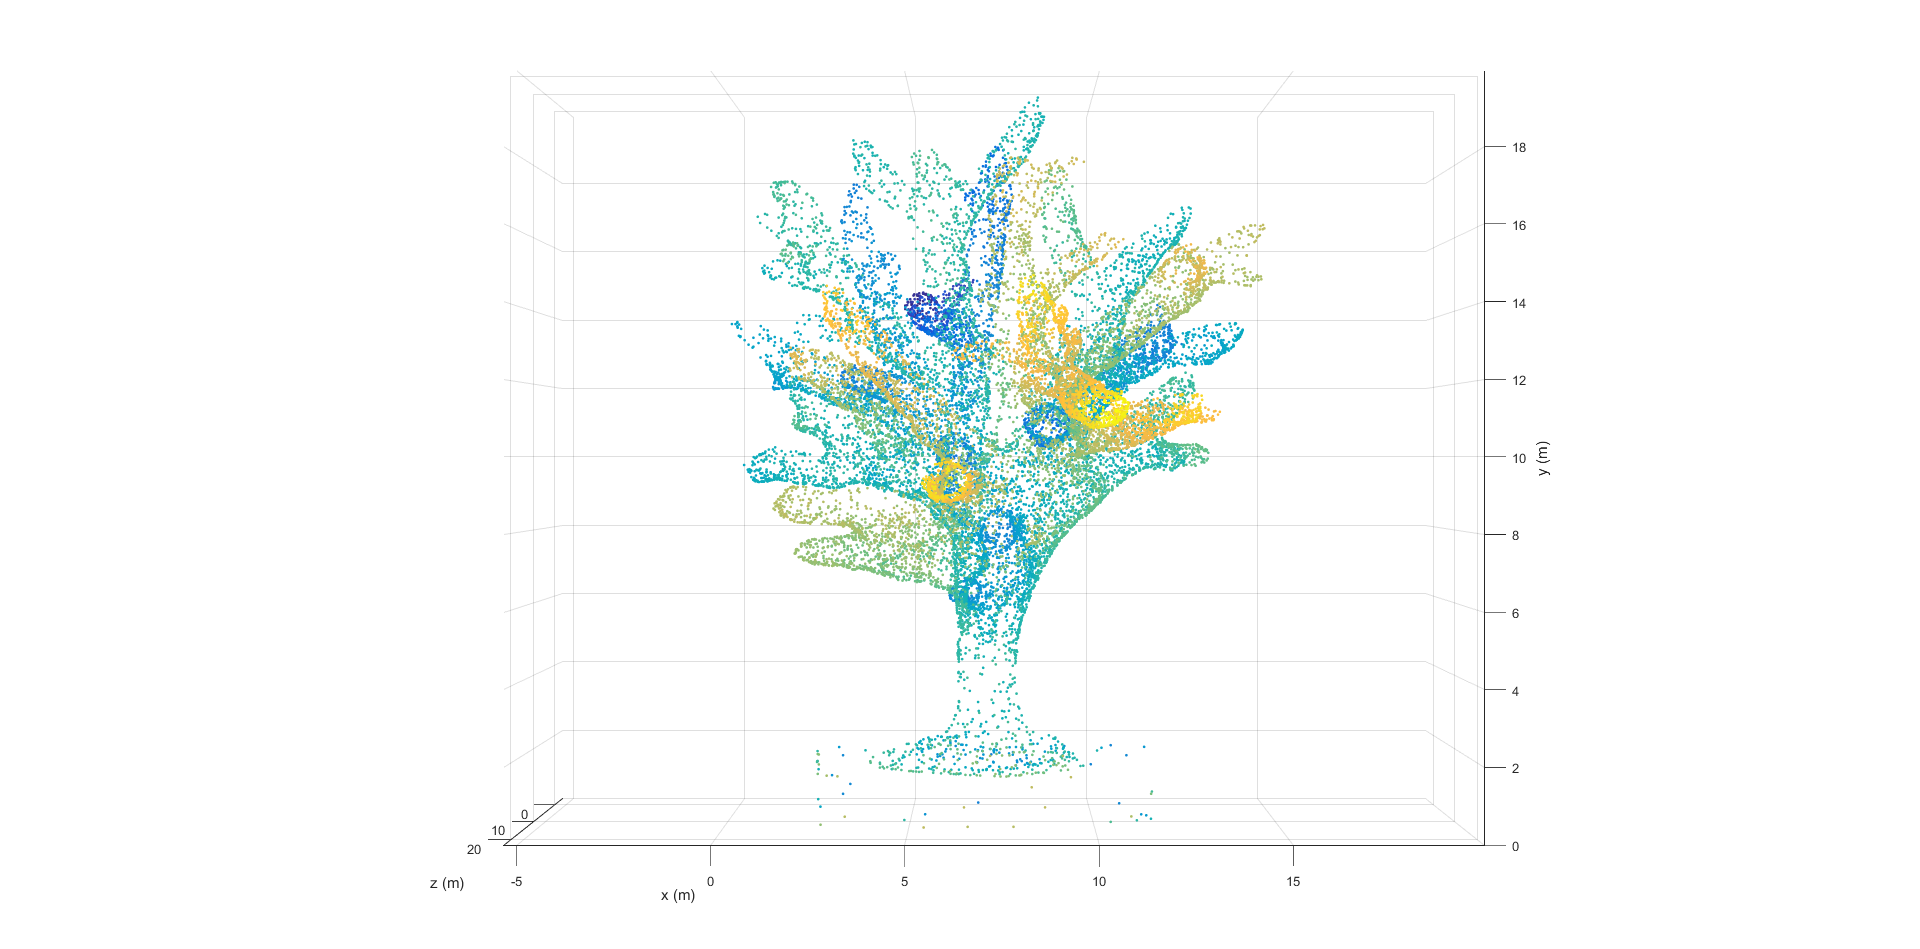
\includegraphics[width=1\textwidth]{images/pointcloud.png}
	\caption{Pointcloud model of a coral.}
	\label{pics:pointcloud}
\end{figure}

\subsubsection{Visualization}
The visualization of the discretized model was done in two steps. The whole configuration space was divided with a certain resolution into single cubical cells. Cells which are occupied by at least one data point from the point cloud were highlighted.    

\begin{figure} [h]
	\centering
	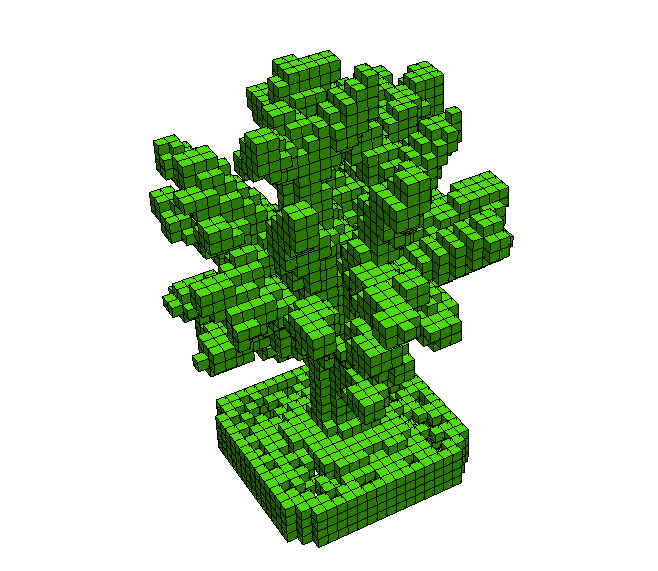
\includegraphics[width=0.5\textwidth]{images/discretized.png}
	\caption{Discretized model of the coral.}
	\label{pics:discretized}
\end{figure}

\subsubsection{Collision-Check}
For collision-checking, the workspace was transformed into a three dimensional matrix according Formulas \ref{eq:occupancy} to \ref{eq:transformation_occupancy}. The size corresponds to the number of cells in the configuration space. Obstacle-free cells carry the value 0 while occupied cells the value 1. 

\begin{equation}
occupancy=zeros(m_{length}/b_{res},m_{width}/b_{res},m_{height}/b_{res})
\label{eq:occupancy}
\end{equation} 

\begin{equation}
[x_{occ},y_{occ},z_{occ}]=[ceil(x_{PC}/b_{res}),ceil(y_{PC}/b_{res}),ceil(z_{PC}/b_{res})]
\label{eq:transformation}
\end{equation}

\begin{equation}
occupancy(x_{occ},y_{occ},z_{occ})=1
\label{eq:transformation_occupancy}
\end{equation} 

\begin{itemize}
	\item
	$m_{length},\,m_{width}$ and $m_{height}$ are the map sizes,
	\item
	$x_{PC},\,y_{PC}$ and $z_{PC}$ are the datapoints from the point cloud,
	\item
	$b_{res}$ is the map resolution respectively the length of a single cubical cell.
\end{itemize}

\section{Object Scanning Route}

The implemented algorithm was used for an object scanning application. For this, the sampling function needed to be rewritten in order to generate solutions within a short amount of time. 

\subsection{Defined Sampling Region}

The RRT* algorithm is not able to generate a feasible paths between all viewpoints (see Figure \ref{pics:viewpoints_paths}) within a relatively short period of time and with a fixed iteration number. This problem was solved by rewriting the sampling function. Instead of sampling in the whole map, the new function samples with 50\% in the goal region (see Figure \ref{pics:sampling}). Therefore, a path is more likely to be found. Furthermore, the program is defined as such that it automatically terminates when all feasible paths are generated. 

\begin{figure} [h]
	\centering
	\includegraphics[width=1\textwidth]{images/sampling_regions.png}
	\caption{Defined sampling region.}
	\label{pics:sampling}
\end{figure}
